\section{Regelungstechnik}
Der Aufbau der Würfelseite stellt ein inverses Pendel dar, folglich handelt es sich um ein instabiles System. Diese Aussage lässt sich leicht an Hand der Pole des Systems überprüfen. Da die Systemmatrix $\bs{A}$ die vollständige Information über das Eigenverhalten enthält, muss diese auch die Pole des Systems beinhalten, welche über die charakteristische Gleichung
\begin{equation}
P^*(s) = |s\cdot \bs{I} -  \bs{A}| = 0
\end{equation}
berechnet werden können. Für das Modell der Würfelseite ergibt sich die folgende charakteristische Gleichung. Die Lösung dieser Gleichung führt wiederum auf die Pole des Systems.
\begin{equation}
P^*(s) = s^3+2,08s^2-76s-20,4=0
\end{equation}
\begin{equation}
p_1=7,89 \hspace{35pt} p_2=-0,27 \hspace{35pt} p_3 = -9,7
\end{equation}
Da der erste Pole einen positiven Realteil besitzt ist das System instabil. Folglich muss ein Regelungskonzept entworfen werden um das System zu stabilisieren. Die primäre Aufgabe des Reglers besteht darin, den Winkel $\varphi$ möglichst rasch in den Sollwert zu überführen. Hierfür wird der Ansatz der Zustandsrückführung gewählt, welcher im folgenden Blockschaltbild dargestellt ist.
\begin{figure}[!h]
\centering
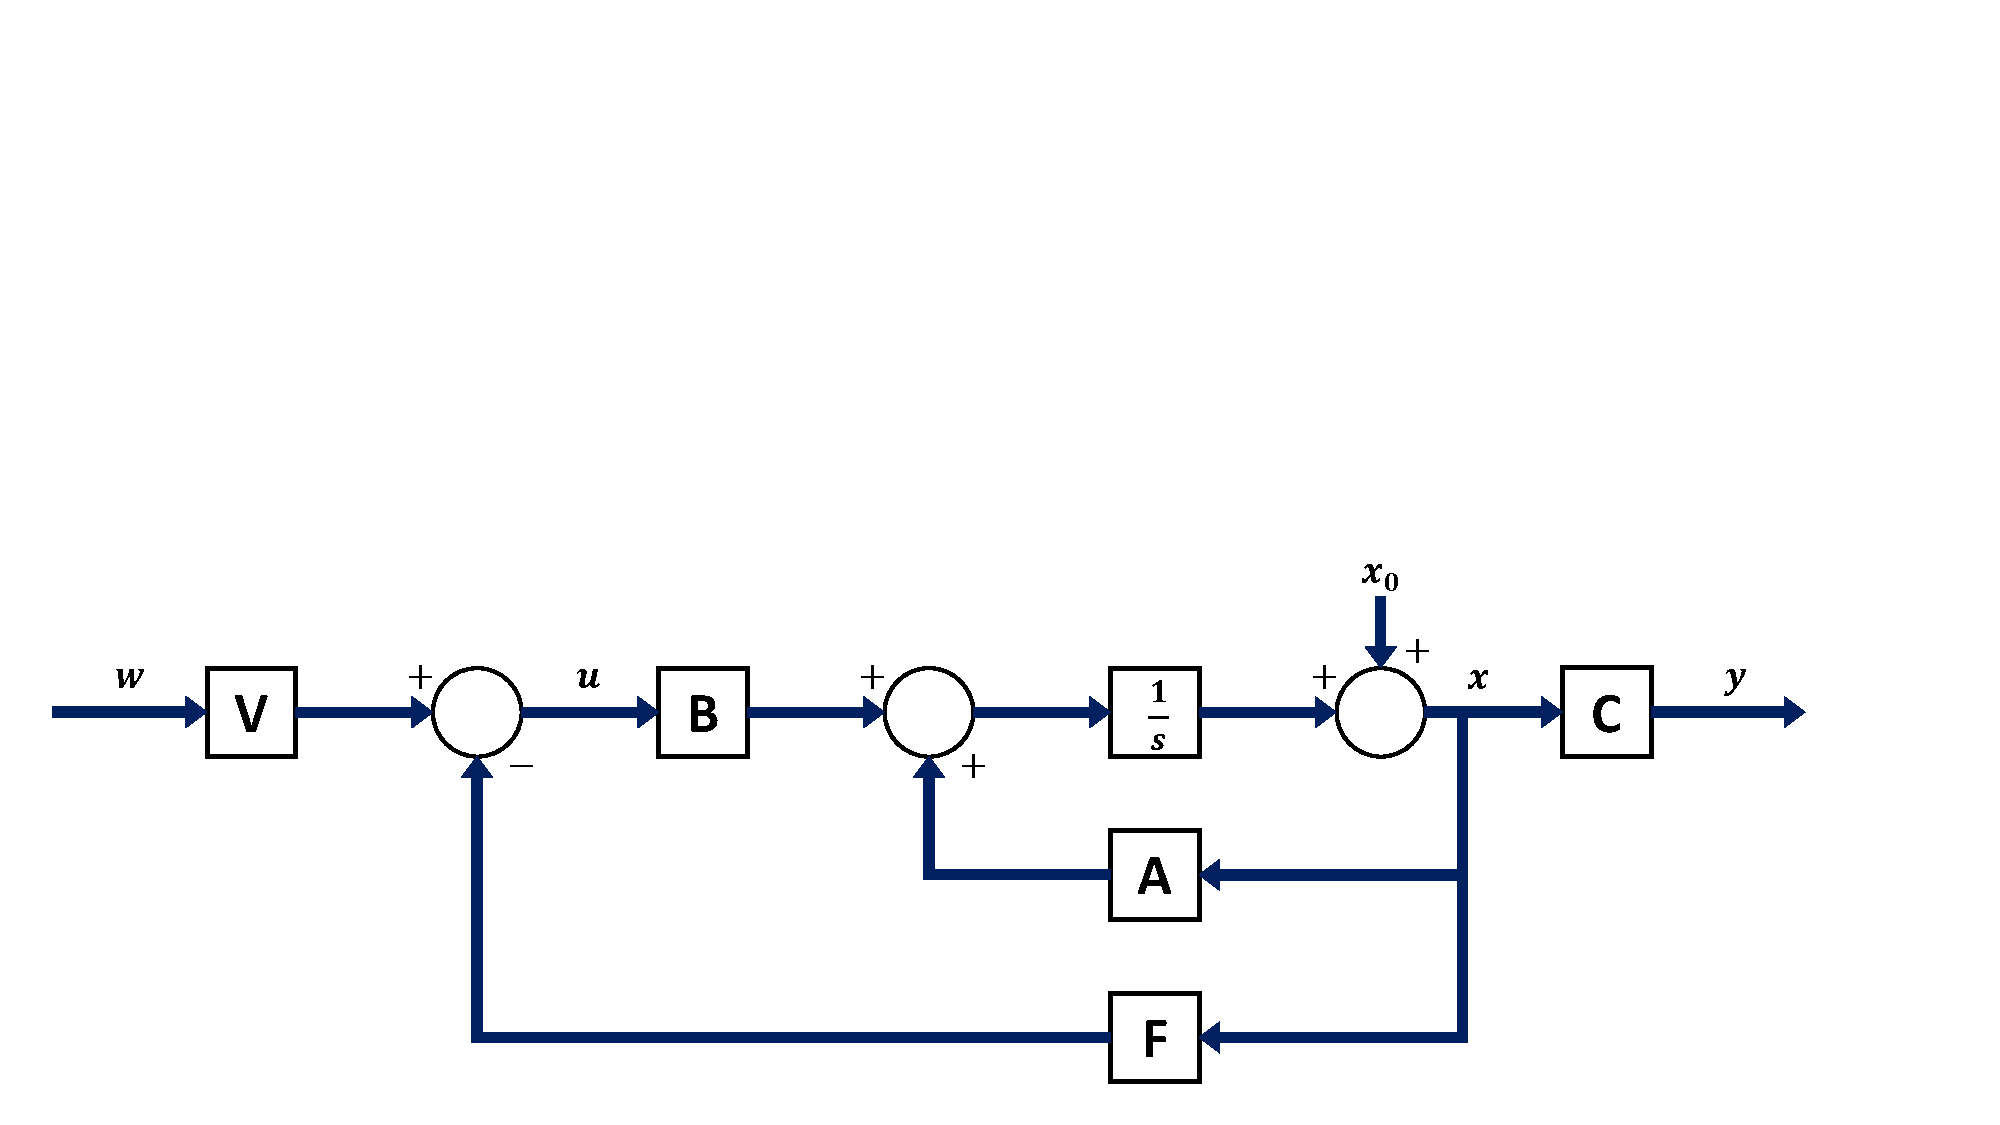
\includegraphics[width=\linewidth,trim={0cm 0cm 2cm 9cm}, clip]{4_Regelungstechnik/img/GRK_1}
\caption{Geschlossener Regelkreis, Quelle: eigene Darstellung, Inhalt aus RT2}
\end{figure}
In dem geschlossenen Regelkreis wurde einerseits der Führungsvektor $\bs{w}$ eingeführt, der mit dem Vorfilter $\bs{V}$ gewichtet wird. Die Funktion des Vorfilters wird später genauer betrachtet. Zusätzlich wird der Zustandsvektor über die Reglermatrix $\bs{F}$ zurückgeführt. Dadurch ergibt sich eine neue Zustandsraumdarstellung.
Die ursprüngliche Eingangsgröße $u$ setzt sich nun aus dem gewichteten Führungsvektor $\bs{V}\bs{w}$ und dem zurückgeführten Zustandsvektor $\bs{F}\bs{x}$ zusammen.
\begin{equation}
u = \bs{V}\bs{w}-\bs{F}\bs{x}
\end{equation}
Einsetzen in die erste Gleichung der Zustandsraumdarstellung führt auf das folgende Ergebnis.
\begin{equation}
\dot{\bs{x}} = \bs{A}\bs{x}+\bs{B}\otimes\bs{V}\bs{w} - \bs{B}\otimes\bs{F}\bs{x} = (\bs{A}-\bs{B}\otimes\bs{F})\bs{x}+\bs{B}\otimes\bs{V}\bs{w}
\end{equation}
Somit ergeben sich für den geschlossenen Regelkreis die neue Systemmatrix $\bs{A}_g=\bs{A}-\bs{B}\otimes\bs{F}$ und Eingangsmatrix $\bs{B}_g=\bs{B}\otimes\bs{V}$. Die zweite Gleichung der Zustandsraumdarstellung bleibt unverändert.
\begin{equation}
\bs{C}_g = \bs{C} \hspace{35pt} \bs{D}_g=\bs{D}
\end{equation}

\subsection{Entwurf der Reglermatrix $\bs{F}$}
Das Eigenverhalten des neuen Systems wird nun von der Systemmatrix $\bs{A}_g$ bestimmt. Deren Pole können ebenfalls über die charakteristische Gleichung
\begin{equation}
P^*(s) = |s\cdot\bs{I}-\bs{A}_g| = 0
\end{equation}
berechnet werden. Somit besteht die erste Aufgabe des Reglerentwurfes darin die Filtermatrix $\bs{F}$ so zu entwerfen, dass alle Pole des geschlossenen Reglekreises in der linken Halbebene liegen, wodurch die Stabilität des Systems gegeben ist. Hierfür wird der Ansatz des optimalen Zustandreglers nach dem quadratischen Gütekriterium gewählt. Das heißt, dass ein Gütekriterium $I$ gewählt wird, welches durch die Wahl von $\bs{F}$ minimiert werden muss.
\begin{equation}
I = \int^{\infty}_0 (\bs{x}^T\bs{Q}\bs{x}+\bs{u}^T\bs{R}\bs{u})dt \overset{!}{=}min
\end{equation}

\textcolor{red}{Einschub wie dieses Optimierungsproblem gelöst werden kann}

Die positiven Matrizen $\bs{Q}$ und $\bs{R}$ dienen zur Gewichtung des Zustand- und Eingangsvektors. Die Wahl der Gewichtungsmatrizen liegt bei dem Entwickler und bietet die Beeinflussung des dynamischen Verhaltens des Regelkreises. In diesem Anwendungsfall werden Diagonalmatrizen verwendet, deren Diagonalelemente über die maximal zulässigen Werte der Zustands- und Eingangsgrößen festgelegt werden.
\begin{equation}
\bs{Q} = \begin{pmatrix}
(\varphi_{max})^{-2} & 0 & 0 \\
0 & (\dot{\varphi}_{max})^{-2} & 0 \\
0 & 0 & (\dot{\psi}_{max})^{-2}
\end{pmatrix}
\hspace{35pt}
\bs{R} = \begin{pmatrix}
({T_M}_{max})^{-2}
\end{pmatrix}
\end{equation}
Dadurch ergeben sich die folgenden Werte für die Reglermatrix $\bs{F}$.
\begin{equation}
\bs{F}=\begin{pmatrix}
-0,9120 & -0,0773 & -0,0001
\end{pmatrix}
\end{equation}
Mit Hilfe der Filtermatrix kann nun die charakteristische Gleichung des geschlossenen Regelkreises gelöst werden, wodurch man die Pole des Systems erhält.
\begin{equation}
|s\cdot \bs{I}-\bs{A}_g| = 0 \hspace{15pt}\rightarrow\hspace{35pt} p_1 = -0.117 \hspace{35pt} p_{2,3} = -11.9 \pm6.55j
\end{equation}
Da alle Pole einen negativen Realteil besitzen ist die Stabilität des Systems nachgewiesen.

\subsection{Entwurf des Vorfilters $\bs{V}$}
Die zweite Aufgabe des Reglerentwurfs besteht darin das Vorfilter $\bs{V}$ so zu entwerfen, dass im stationären Zustand $\dot{\bs{x}}=0$ der Führungs- und Ausgangsvektor übereinstimmen.
\begin{equation}
\label{VEntwurf_eq1}
\bs{w}=\bs{y}=\bs{C}\cdot\bs{x}
\end{equation}
Im stationären Zustand gilt für die erste Gleichung der Zustandsraumdarstellung:
\begin{equation}
\dot{\bs{x}}= (\bs{A}-\bs{B}\otimes\bs{F})\bs{x}+\bs{B}\otimes\bs{V}\bs{w}=0 \hspace{15pt}\rightarrow\hspace{15pt} \bs{x} = (\bs{A}-\bs{B}\otimes\bs{F})^{-1} (\bs{B}\otimes\bs{V})\bs{w}
\end{equation}
Durch Einsetzen der Lösung in (\ref{VEntwurf_eq1}) erhält man das folgende Ergebnisse.
\begin{equation}
\bs{w}=\bs{C}(\bs{A}-\bs{B}\otimes\bs{F})^{-1} (\bs{B}\otimes\bs{V})\bs{w}
\end{equation}
Aus diesem Ausdruck ist leicht zu erkennen, dass die folgende Gleichung gelten muss.
\begin{equation}
\bs{C}(\bs{A}-\bs{B}\otimes\bs{F})^{-1} (\bs{B}\otimes\bs{V}=\bs{I} \hspace{15pt}\rightarrow\hspace{15pt} \bs{V} = [\bs{C}(\bs{B}\otimes\bs{F}-\bs{A})^{-1}\bs{B}]^{-1}
\end{equation}
Berechnet man $\bs{V}$ nach der obigen Formel erhält man für das Vorfilter die folgenden Werte.
\begin{equation}
\bs{V} = \begin{pmatrix}
0 & 3,316\cdot 10^{-5}
\end{pmatrix}
\end{equation}
Das Verschwinden des ersten Elements des Vorfilters lässt sich damit begründen, dass das System nur bei dem Führungswert $\varphi=0$ stabilisiert werden kann. Die erste Bewegungsgleichung
\begin{equation}
(I^{K/O}+I^{R/M}+m_R\cdot l_{AB}^2)\cdot \ddot{\varphi} = m_G \cdot g \cdot l_{AC} \cdot s_{\varphi} - C_{\varphi} \cdot \dot{\varphi} - I^{R/M} \cdot \ddot{\psi}
\end{equation}
zeigt, dass durch die Gravitation ein konstantes Moment ensteht falls $\varphi\neq 0$ gilt. Somit muss der Motor eine konstante Beschleunigung der Schwungmasse erzeugen um $\varphi$ auf dem Führungswert zu halten. Diese Beschleunigung bedeutet allerdings, dass der Zustand $\dot{\psi}$ divergiert und das System somit nicht stabil sein kann.

\subsection{Entwurf eines kaskadierten Regelkreises}
Nach dem Entwurf des stabilen Systems, ist dessen Verhalten in Abhängigkeit von dem Anfangszustand $\bs{x}_0$ von Interesse. Der Führungsvektor ist dabei konstant $\bs{w}=\begin{pmatrix}
0 & 0 
\end{pmatrix}^T$. Das bedeutet, dass die Würfelseite in der aufrechten Position stehen soll und die Schwungmasse dabei zum Stillstand kommt. Um die Endwerte für diesen Führungsvektor zu bestimmen wird die Zustandsraumdarstellung des geschlossenen Regelkreises in den Bildbereich transformiert.
\begin{equation}
s\cdot\bs{X}(s) - \bs{x}_0 = (s\cdot\bs{I}-\bs{A}_g)\bs{X}(s) \hspace{15pt}\rightarrow\hspace{15pt} \bs{X}(s) = (s\cdot\bs{I}-\bs{A}_g)^{-1}\bs{x}_0
\end{equation}
Mit Hilfe des Endwertsatzes
\begin{equation}
x(\infty)=\lim_{s\rightarrow 0} s\cdot \bs{X}(s)
\end{equation}
können die Endwerte des Zustandvektors berechnet werden. Voraussetzung hierfür ist, dass die Endwerte existieren. Dies ist allerdings durch die Stabilität des Systems gegeben. Für den Fall, dass der Führungsvektor $\bs{w}$ verschwindet, konvergieren die Zustandsgrößen gegen null.
\begin{equation}
x(\infty)=\lim_{s\rightarrow 0} s\cdot \bs{X}(s) = \begin{pmatrix}
0 \\ 0 \\ 0
\end{pmatrix}
\end{equation}
Allerdings zeigt eine Simulation bei $\bs{x}_0=\begin{pmatrix}
5^\circ & 0 & 0
\end{pmatrix}^T$, dass lediglich der Winkel $\varphi$ in kurzer Zeit gegen Null konvergiert. Die Geschwindigkeit $\dot{\psi}$ benötigt einen verhältnismäßig großen Zeitraum um abzuklingen.
\begin{figure}[!h]
\centering
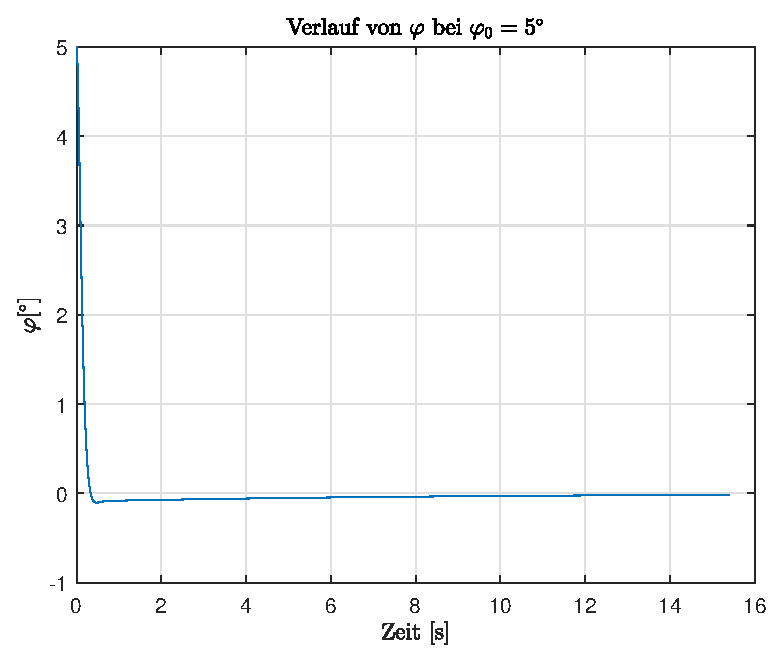
\includegraphics[width=0.45\linewidth]{4_Regelungstechnik/img/x0_phi}
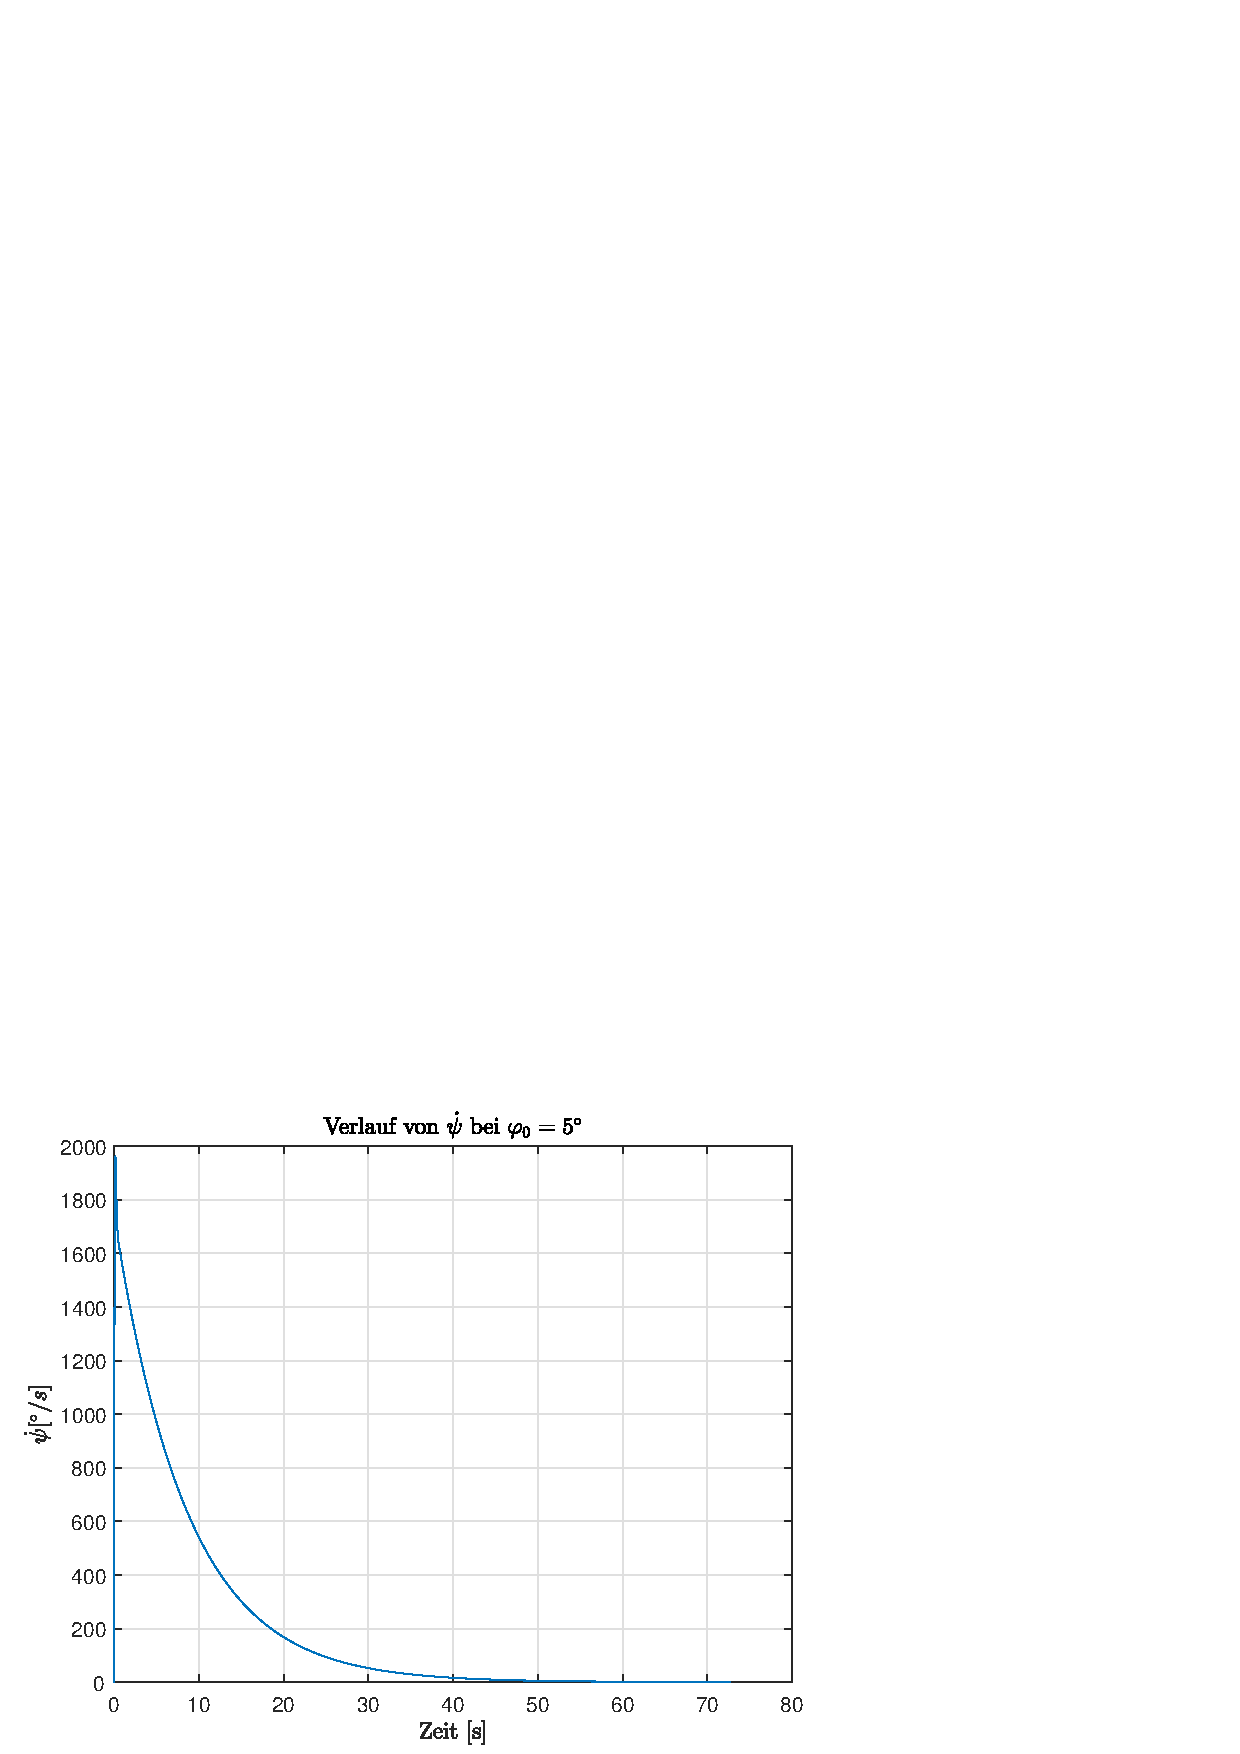
\includegraphics[width=0.45\linewidth]{4_Regelungstechnik/img/x0_psi__d}
\caption{Verlauf von $\varphi$ und $\dot{\psi}$, Quelle: eigene Darstellung}
\end{figure}
Das sekundäre Regelungsziel besteht darin, die nötige Zeit für die Konvergenz von $\dot{\psi}$ zu reduzieren. Da der Führungsvektor entfällt ist für das Verhalten des geschlossenen Regelkreises nur die Fundamentalmatrix von Bedeutung. Die Übertragungsmatrix beschreibt lediglich das Verhalten des Systems auf ein Eingangssignal und ist somit hier nicht relevant. Außerdem wird hier lediglich das Produkt der Ausgangsmatrix $\bs{C}$ und der Fundamentalmatrix $\Phi$ betrachtet, da sich die Zustandsgröße $\dot{\varphi}$ aus dem Verlauf von $\varphi$ ergibt.
\begin{equation}
\bs{C}\cdot\bs{\Phi}(s) = \begin{pmatrix}
\frac{2,54s^2+60,9s-1,3}{2.54s^3+60,9s^2+478s+55,1} &
\frac{6,87s-2,02}{6,87s^3+165s^2+1300s+149} &
\frac{-0,53}{55s^3+1320s^2+10400s+1190} \\
\frac{1720s + 13900}{0,22s^3+5,16s^2+40,5s} &
\frac{147s+1720}{0,22s^3+5,16s^2+40,5s+4,66} &
\frac{0,22s^2+5,22s+40,6}{0,22s^3+5,16s^2+40,55s+4,66}
\end{pmatrix}
\end{equation}
Das Zeitverhalten des geschlossenen Regelkreises wird durch die Pole vorgegeben. Diese sind in der Fundamentalmatrix enthalten. Hierbei gilt, dass ein Pol, der weit von der imaginären Achse entfernt ist zu einem schnelleren Systemverhalten führt. Bei Systemen mit mehreren Polen gibt das Dominanzmaß $D_i$ den relativen Einfluss der Pole wieder. Hierfür werden die Teilübertragungsfunktionen bzw. Elemente der Fundamentalmatrix in Partialbrüche umgeformt.
\begin{equation}
G(s) = \sum^i \frac{A_i}{s-p_i}
\end{equation} 
\begin{equation}
D_i = \vert\frac{A_i}{p_i}\vert
\end{equation}

Die folgende Tabelle zeigt die Dominanzmaße der drei Pole
\begin{equation}
p_{1,2} = -11.9+6.55j \hspace{35pt} p_3 = -0.117
\end{equation}
in den Elementen der Fundamentalmatrix. Diese geben wieder, wie stark Zusammenhang zwischen Ausgangsvektor und Anfangswert des Zustandsvektors von den verschiedenen Polen beeinflusst wird.
\begin{table}
\centering
\begin{tabular}{c|c|c|c}

 & $\varphi_0$ & $\dot{\varphi}_0$ & $\dot{\psi}_0$ \\ 
\hline
$\varphi$ & $D_{1,2}=0.078 \hspace{15pt} D_3=0.155$ & $D_{1,2}=0.006 \hspace{15pt} D_3=0.019$ & $D_{1,2}=4\cdot10^{-6} \hspace{15pt} D_3=4.5\cdot10^{-6}$ \\
\hline
$\dot{\varphi}$ & $D_{1,2}=24.6 \hspace{15pt} D_3=2984$ & $D_{1,2}=1.86 \hspace{15pt} D_3=371$ & $D_{1,2}=0.001 \hspace{15pt} D_3=8.71$ 

\end{tabular}
\end{table}
Aus der Tabelle ergibt sich, dass der dominierende Pol des Systems $p_3=-0.117$ ist. Dessen kleiner Realteil führt zu einer langsamen Eigenbewegung. Allerdings fließen das komplex konjugierte Polpaar $p_{1,2}=-11.9\pm6.55j$ nach wie vor in den Verlauf von $\varphi$ ein. Dadurch lässt sich die relativ rasche Konvergenz von $\varphi$ gegen den Endwert erklären. 
Der Verlauf der Zustandsgröße $\dot{\psi}$ wird allerdings von dem Pol $p_3$ dominiert. Das Dominanzmaß der Poolpares $p_{1,2}$ ist um mehrere Potenzen geringer und beeinflusst somit den Verlauf von $\dot{\psi}$ kaum. Dies erklärt wiederum das langsame Konvergenzverhalten von $\dot{\psi}$.

Folglich muss entweder die Lage der Pole oder deren Dominanzmaß verändert werden um die Systemdynamik zu beeinflussen. Hierfür wird eine kaskadierte Regelung verwendet, das heißt der Ausgangsvektor des geschlossenen Regelkreises wird auf den Führungsvektor zurückgeführt.
\begin{figure}[!h]
\centering
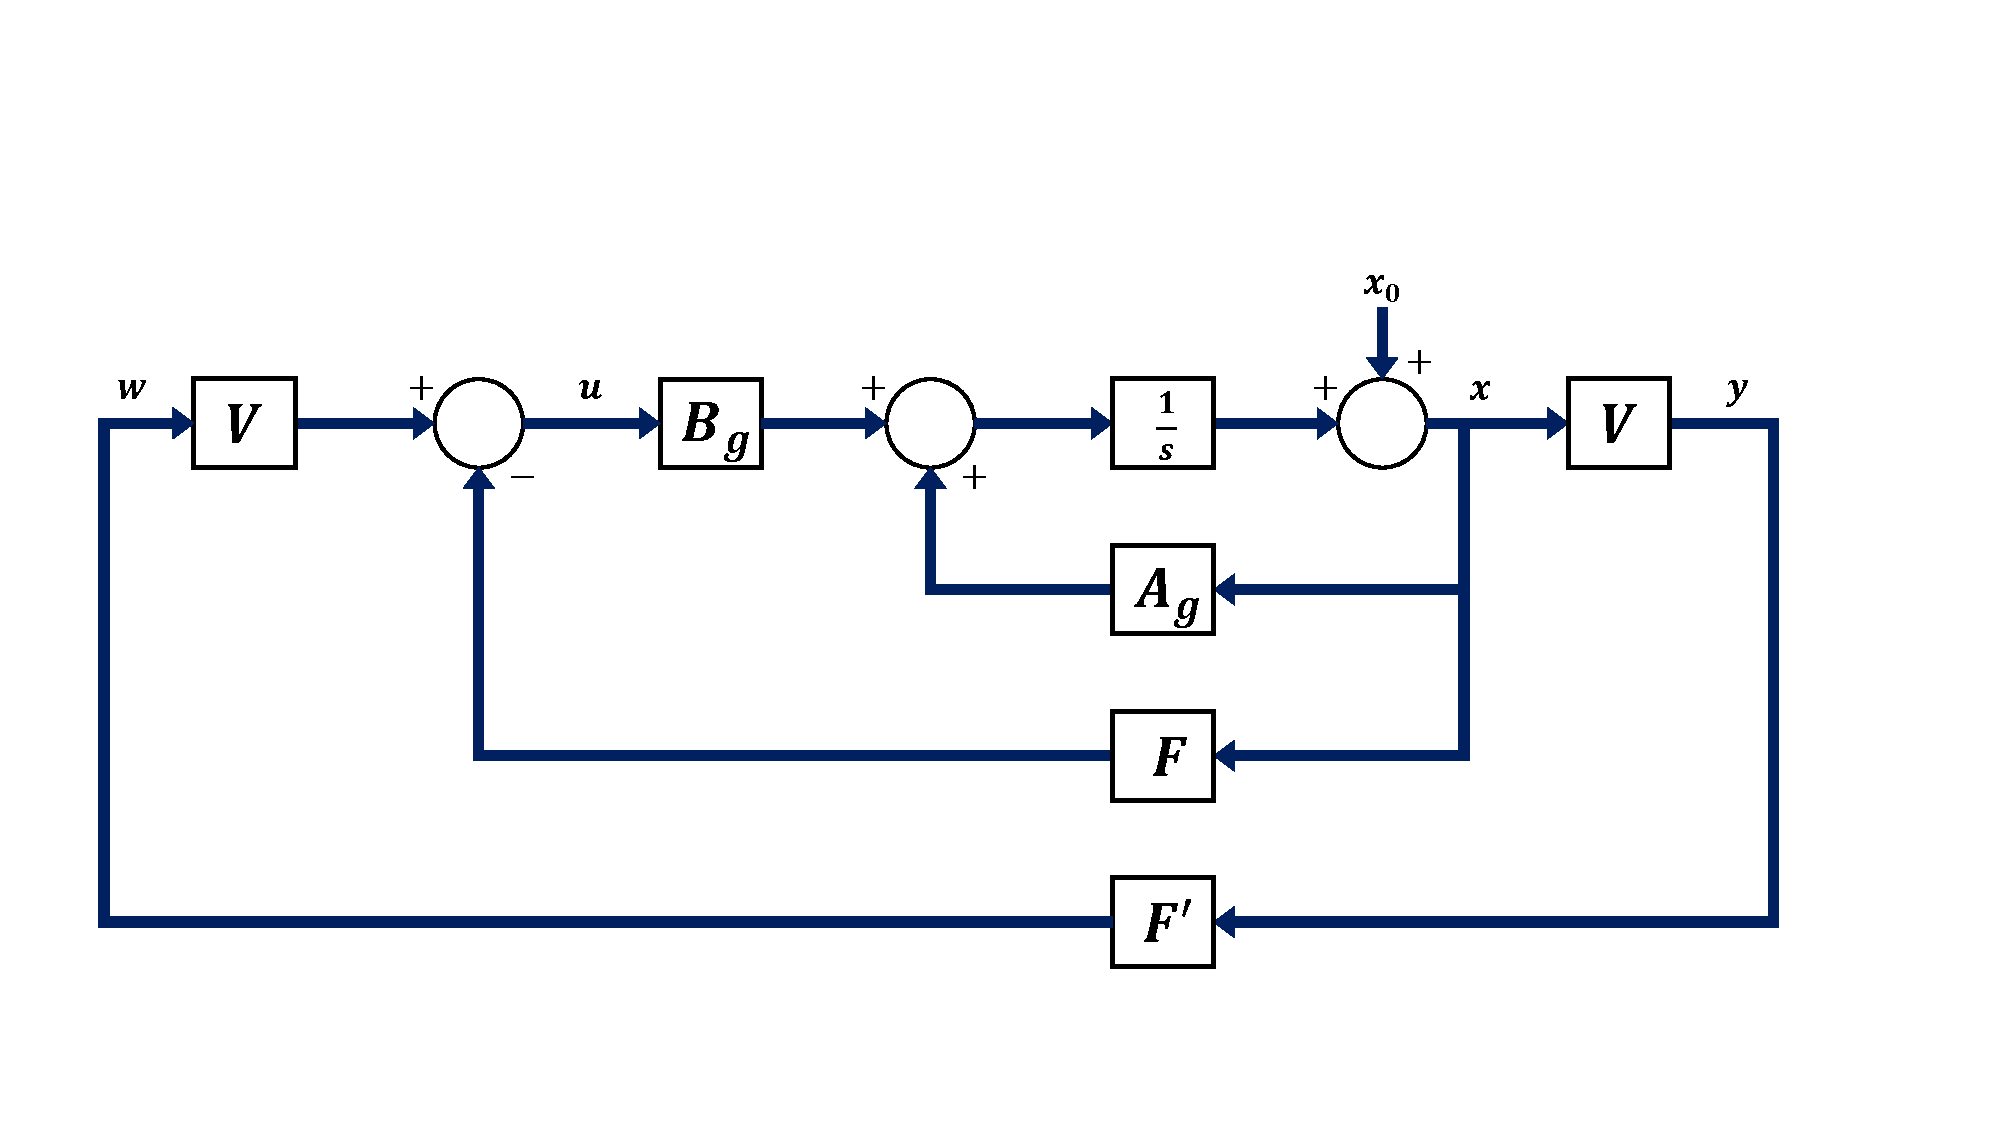
\includegraphics[width=0.9\linewidth,trim={0cm 2cm 2cm 4.5cm}, clip]{4_Regelungstechnik/img/GRK_2}
\caption{Kaskadierter Regelkreis, Quelle: eigene Darstellung}
\end{figure}
Aus dem Blockschaltbild ist zu erkennen, dass für den Führungsvektor $\bs{w}$ der folgende Zusammenhang gilt.
\begin{equation}
\bs{w}=\bs{F}'\bs{y}
\end{equation}
Durch Einsetzen in die erste Gleichung der Zustandsraumdarstellung ergibt sich:
\begin{equation}
\dot{\bs{x}}=\bs{A}_g\bs{x}+(\bs{B}_g\otimes\bs{F}')\bs{y} = (\bs{A}_g+\bs{B}_g\otimes\bs{F}'\otimes\bs{C})\bs{x} = \bs{A}_c\bs{x}
\end{equation}\textcolor{red}{diadische Produkte beweisen, ist vlt nicht ganz richtig}
Die zweite Reglermatrix $\bs{F}'$ setzt sich aus zwei wählbaren und zwei Nullelementen zusammen. Der Grund dafür, dass zwei Elemente der Matrix verschwinden liegt darin, dass der Wert für $\varphi$ im Führungsvektor keinen Einfluss auf das System hat, da der Vorfilter diesen nicht gewichtet.
\begin{equation}
\bs{F}'=\begin{pmatrix}
0 & 0 \\ F_1 & F_2
\end{pmatrix}
\end{equation}
Die charakteristische Gleichung des kaskadierten Regelkreises hängt von der Reglermatrix $\bs{F}'$ ab. Folglich können auch die Pole des Systems durch die Wahl der Matrixelemente beeinflusst werden.
\begin{equation}
P^*(s) = |s\cdot\bs{I}-\bs{A}_c| = s^3+(24+0,29F_2)s^2+(200+0,41F_2-0,01F_1)s+(22,0-22F_2+10^{-19}) = 0
\end{equation}
\newpage
\textcolor{red}{3Dplots zeigen, dass F1 praktisch irrelevant ist, optimales Erbenis sollte man erreich indem man nur F2 betrachtet und den Betrag der Pole+Dominanzmaß mit dem Stabilitätsrand vergleicht, optimale Lösung ist die Kombination aus maximalen Betrag aller Pole die nach wie vor stabil sind, Frage ob das noch praktisch analysbar zu lösen ist oder man einfach das Optimum aus den Plots rausnimmt}

Die folgenden Darstellung zeigen den Verlauf der Zustandsgrößen bei $\bs{x}_0=\begin{pmatrix}
5^\circ & 0 & 0
\end{pmatrix}^T$ des kaskadierten Regelkreises. Für die zweite Reglermatrix wurden die Werte $F_1=0$ und $F_2=-17$ verwendet.
\begin{figure}[!h]
\centering
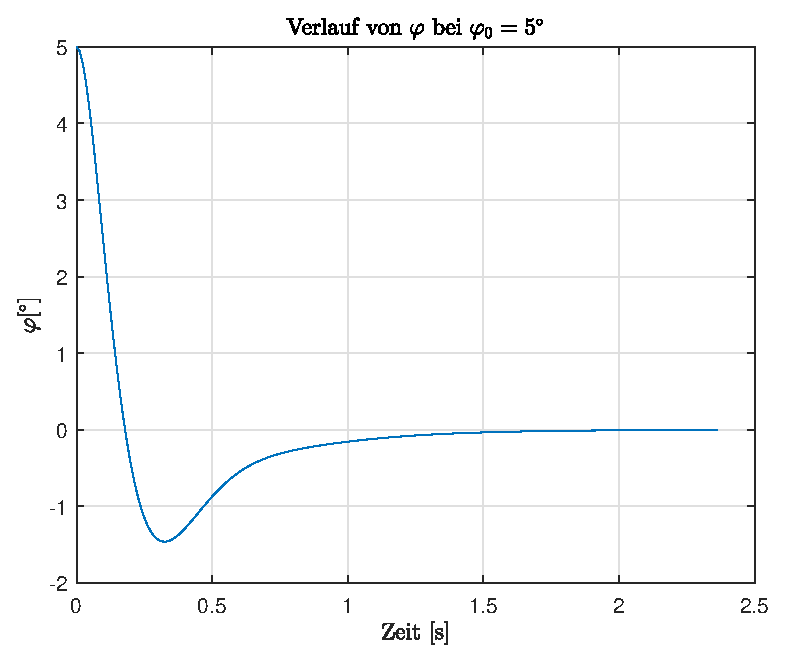
\includegraphics[width=0.45\linewidth]{4_Regelungstechnik/img/x0_phi_kaskadiert}
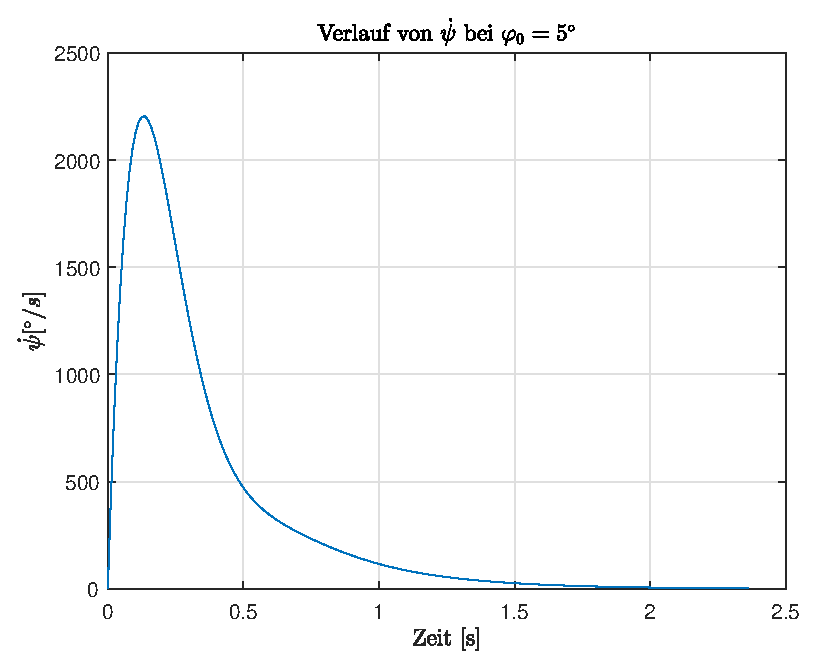
\includegraphics[width=0.45\linewidth]{4_Regelungstechnik/img/x0_psi__d_kaskadiert}
\caption{Verlauf von $\varphi$ und $\dot{\psi}$, Quelle: eigene Darstellung}
\end{figure}